%% LyX 1.3 created this file.  For more info, see http://www.lyx.org/.
%% Do not edit unless you really know what you are doing.
\documentclass[english]{article}
\usepackage[T1]{fontenc}
\usepackage[latin1]{inputenc}
\usepackage{graphicx}

\makeatletter

%%%%%%%%%%%%%%%%%%%%%%%%%%%%%% LyX specific LaTeX commands.
%% Bold symbol macro for standard LaTeX users
\newcommand{\boldsymbol}[1]{\mbox{\boldmath $#1$}}


\usepackage{babel}
\makeatother
\begin{document}

\title{Ph.D. Report}


\author{Julian Brown}

\maketitle

\section{Personal information}

I am (will be) a second-year Ph.D. student in the Languages and Architecture
group. My supervisor is Prof. David May.


\section{Achievements}


\subsection{First six months}

The first six months or so of my Ph.D. I was working in the Computer
Vision group under Prof. Barry Thomas.


\subsection{Last six months}

\begin{itemize}
\item Moved to Languages and Architecture group
\item Continued some work on binary translation from my final-year university
project (see below)
\item Design proposal for new ISA, targeted at dynamic optimisation
\item Read some papers
\item Attempted to obtain familiarity with up-to-date processor and compiler
technology
\end{itemize}

\subsection{Next six months}

\begin{itemize}
\item Pending further discussion
\end{itemize}

\section{Background}

The research I intend to carry out is in the field of dynamic optimisation.

To achieve this aim, a new instruction-set architecture (ISA) will
be developed, with the specific aims of ease of program analysis,
and with features to reduce the overhead for run-time code modification
to a minimum.

The starting point of this research is in an emulation system, which
though not trying to solve exactly the same problem, has given a fair
amount of insight into what the problems are in trying to analyse
and optimise code as it is running. An overview of this system is
given below for informational purposes, and to give some backup to
the reasoning behind some of the new architecture features I am proposing.

The work which needs to be completed is as follows. Firstly, the new
architecture (provisionally named {}``Chameleon'') needs to be finalised
(a draft version is described below). Secondly, a toolchain needs
to be developed for the purposes of sourcing binaries for the architecture.
It is anticipated that suitable modifications to the `gcc' compiler
can be made. Also, an execution environment needs to be developed,
which is accurate enough to model the estimated performance of a hardware
implementation of Chameleon. Only then can dynamic optimisation techniques
be tested and developed.

It will be useful to try to duplicate as little work as possible before
that point is reached. Existing projects such as SimpleScalar%
\footnote{http://www.simplescalar.com/%
} or SimOS%
\footnote{http://simos.stanford.edu/%
} might be exploited to avoid implementing an entire realistic virtual
machine.


\section{Dynamic Optimisation}


\subsection{What is dynamic optimisation?}

Traditional compiler optimisations attempt to improve the object code
produced from a high-level source program using a variety of methods
-- by altering the structure of code, removing redundancy, exploiting
particular machine features, and so on. These optimisations typically
take place during various stages of compilation: on the source program
directly (eg, loop transformations), on some compiler intermediate
representation, or on the binary code itself (eg, peephole optimisation).

Dynamic optimisation typically operates directly on object code, guided
by statistical data gathered from program execution. There are several
ways in which dynamic optimisation might enable higher performance
for executed code than traditional optimisations which take place
at compile-time.

Firstly, the code can be optimised in such a way to take full advantage
of the available functional units, cache heirarchy, etc. of the machine
which it's run on. The only way to do this with a traditional compiler
is to ship multiple versions of the same binary, and even then, new
machines might not be taken advantage of fully.

Secondly, program behaviour can be monitored continuously, as its
behaviour changes due to the data it is working on or the conditions
of its environment. This monitoring should enable code to be reordered,
specialised, complex control flow to be linearised, etc. to increase
overall performance.

Thirdly, certain constructs can be simplified at run time in a way
which is impossible, impractical or inefficient at compile-time. This
includes calls to functions in shared libraries, which can be rewritten
to point directly to the code (or even inlined completely, for small
functions), and indirect function calls (eg, method invocations in
object-oriented code), which can be turned into direct function calls,
which are typically faster on modern processors.


\subsection{Dynamic vs profile-driven optimisation}

There has been much focus recently on profile-driven optimisation
techniques. In fact, certain new processor designs are practically
dependent on such techniques to achieve their best performance (eg,
Intel's IA-64 \cite{Hazelwood}), due to their reliance on static
instruction scheduling, rather than the dynamic instruction scheduling
which has become commonplace in superscalar designs.

There are two main problems with the profile-driven approach. The
first is that a program must be run with a set of `typical' data at
compile time, and such data is not always available, or the program
will be run on such diverse data that it is not possible to pinpoint
a particular data set to optimise on. The second problem is more pragmatic,
in that it is difficult to persuade developers to develop and ship
code using profile-driven compilation, since it adds another two (potentially
time-consuming) stages to the build process. Moreover, problems with
compilers in the past have led to much commercial software being shipped
with optimisations turned off altogether.

Dynamic optimisation solves each of these problems. In the latter
case, developers do not need to perform extra profile-gathering and
optimisation passes. In the former case, since code can adapt to whatever
data it is running on at the time, there is no need to create contrived
`typical' data sets. Even data which changes in character as a program
is running can be handled, as the program may adapt to those changes.


\subsection{Existing work}

An amount of work has been done on various related topics, feedback-directed
optimisation, dynamic optimisation, dynamic recompilation. Some projects
are briefly dissected below.


\subsubsection{HP Dynamo}

One of the best-documented attempts at dynamic optimisation is Hewlett
Packard's Dynamo. The outcome of their research was to successfully
reduce the running time of native HP/UX binaries running on PA-RISC
powered workstations, despite using an (initially) software emulation-based
approach.

Originally, the aim of their research was to investigate how feasably
binary translation can be used to execute non-native program binaries
at native speeds. For ease of implementation or otherwise, they started
out with the same architecture (PA-RISC) for their source and target
codes, and to their surprise native binaries would sometimes actually
improve in execution speed, sometimes by 20\% or more.

Dynamo executes entirely in user space on unmodified hardware. Much
like many dynamic recompilation systems, it starts out by always \emph{emulating}
the code it's running. It profiles code as it runs it, building up
a \emph{fragment cache} of sections of code which are executed frequently.
These fragments are `traces' from the original execution of the code
-- that is, they linearise complicated control flow, turning it into
straight-line code. This can be handled more efficiently by the CPU's
prefetch hardware and instruction cache.

The other way Dynamo gains an advantage over statically-optimised
code is by using its own lightweight optimiser. Since optimisation
is done at run-time, optimisations themselves must be done very quickly.
The optimisations attempted include optimisations across procedure
call/return boundaries and indirect branches or virtual function calls.

Since Dynamo operates on native binaries, if at any point it decides
that too much time is being spent in re-optimisation, it can ``bail
out'' and return control to the native processor. This obviously isn't
possible if non-native binaries are being used.


\subsubsection{Morph}

Harvard University's Morph is a project which attempt to perform optimisation
({}``morphing'') on annotated binary files between loading and execution.
The Morph design is based on three requirements. Firstly, optimisation
should be done on the same machine that the code is to be executed
on, so that profile data is meaningful. Secondly, no source code should
be required for the optimisation, as this is not usually shipped with
commercial software due to its proprietary nature. Thirdly, optimisation
should be entirely transparent to the end-user.

Morph is comprised of five components -- the Morph back-end, Morph
Monitor, Morph Editor, Morph Manager, and a tool called Post Morph.
The Morph back-end is an add-on to SUIF which produces executable
code along with annotations necessary to perform re-optimisation.
The Morph Monitor runs constantly as part of the operating system
to gather profile data. The Morph Editor is a component built into
the SUIF research compiler that performs optimisations on the intermediate
representation produced by SUIF and produces an executable. The Morph
Manager is an off-line system component which makes decisions about
when to re-optimise programs based on profile data collected by the
Morph Monitor.

Since optimisation is performed off-line, dynamic usage patterns of
software cannot be exploited with the Morph system.


\subsubsection{Spike}

Spike \cite{2} is a tool from Digital (Compaq, HP) to optimise programs
for Alpha/Windows NT. Like Morph, profiling is done online and optimisation
is done offline, on binary code. The Spike system can optimise large
applications made up from many executables and DLLs, without needing
source code. According to the spiel, program code is split between
two varieties, loop-intensive programs and call-intensive programs.
Traditional compiler technology is geared towards supporting the former
more strongly, whereas GUI applications typically fall into the second
camp.

Optimisations performed are code layout, to improve locality and reduce
the number of instruction cache misses, and hot-cold optimisation
\cite{CL 96}, which optimises the frequent paths through a procedure
at the expense of the infrequently executed paths. The latter is claimed
to be particularly effective in optimising procedures with complex
control flow and high procedure call overhead.


\subsubsection{Jalapeno}

From IBM Research's web page, Jalapeno is a Java virtual machine with
the following features:

\begin{itemize}
\item The entire virtual machine (VM) is implemented in Java
\item The VM utilises two compilers and no interpreter
\item A family of parallel, type-exact garbage collectors
\item A lightweight thread package with compiler-supported preemption
\item An aggressive optimizing compiler, and
\item A flexible online adaptive compilation infrastructure
\end{itemize}
Probably the most interesting thing about Jalapeno from the point
of view of this project is the way it optimises frequently-executed
code more than infrequently-executed code, using statistical sampling
of the program counter.


\subsubsection{Transmeta Crusoe}

Transmeta's Crusoe%
\footnote{http://www.transmeta.com/%
} processor is designed with dynamic code translation in mind. It includes
hardware support for precise exceptions and speculation in rescheduled
code (shadow registers), optimization of memory operations (alias
hardware), and self-modifying code (a ``translated\char`\"{} bit in
the MMU). And of course it works on non-native binaries, executing
IA-32 code on a VLIW processor core.

Crusoe's method of operation is otherwise similar to that used by
various emulation systems. It starts out emulating code, then for
frequently executed sections it does a `rough' translation to its
own native (VLIW) code. These translations are cached and further
optimised over time the more they are executed. By this method the
designers claim that performance comparable to a modern hardware IA-32
implementation is obtained.

The limitation of their approach is their decision to support a legacy
architecture as their source, rather than invent a new architecture
explicitly geared towards enabling dynamic optimisation. This makes
the problem much harder, and also loses a large amount of data from
original source code which would be useful for further optimisation.


\subsection{Limitations of a software-only emulation approach to dynamic optimisation}

I started this research aiming to apply dynamic optimisation techniques
to a dynamically recompiling emulator (for an ARM chip on an IA-32
platform). When writing this sort of emulator (my attempts are described
below), one is not really modelling accurately what a processor actually
does. In fact, it's more like designing an \emph{implementation} of
an instruction-set architecture. This is not useful in all situations
where a traditional emulator might be used -- say, coverification
of hardware models designed around the processor, but is sufficient
to run operating system-level software. In many cases, we can fairly
safely take short-cuts on issues such as perfect cycle-timing accuracy
or emulating cache misses without compromising our ability to run
the operating system and its applications, if only because different
real processor implementations might also have different cycle timings
for instructions (eg, Intel's vs AMD's IA-32 offerings), so code is
written to perform timing using other means.

What we must not do is let the state of the virtual machine diverge
from the state of the equivalent real machine over time. For example,
if an emulated leaf subroutine affects the processor flags or a `scratch'
register, we cannot optimise that calculation away, even if the context
in which that leaf subroutine is called is insensitive to the result
of that calculation. We cannot be sure that the subroutine is not
called from elsewhere in such a way that the calculation is vital.
This seems obvious, but severely limits the kind of optimisations
we can perform.

For example, say we were translating code from some hypothetical CISC
processor with eight general-purpose registers available for data
processing. In many cases these are not sufficient to hold all the
temporary values necessary to perform a calculation, so some of them
must instead be stored in memory locations, eg the stack. If we are
translating this code to some RISC architecture with 32 available
registers, it seems desirable to assign some of the stack locations
to registers instead, to make better use of the resources available.
The anticipated problems with this are as follows:

We are looking at the code through a potentially very small `window'.
This leads to a bad case of the `pointer aliasing' problem, whereby
we can't tell if loads or stores to particular memory locations will
affect loads or stores from other memory locations. If we factor out
a store and a load from what we assume to be the stack, and place
the value in a register for the duration, an intermediate load or
store which should affect that value, will not. Transmeta used additional
hardware to help work around this problem, which is not available
if we take a software-only approach. Note it doesn't matter if such
register reallocation would work \emph{most of the time} -- if it
will sometimes fail we simply can't do it.

Similarly, we can't tell (or at least, we probably can't tell) if
a particular load or store points at some volatile memory location,
such as I/O space or a memory location which is touched by code running
under some sort of interrupt. Also similarly, most of the time we
could probably make assumptions, but the rare cases in which we are
wrong would lead to unacceptable program behaviour. Of course, anything
that can be done in hardware can also be done in software, it will
just take longer. If the emulated memory system implements paging
in software, it may well be faster to sometimes use explicit aliasing
checks.

Exceptions are another problem. Exceptions can be divided into two
categories, those which occur asynchronously, where the program counter
location is of little consequence (eg, keyboard interrupts), and those
which occur synchronously, such as page faults. In the latter case,
it's vital that the original state of the processor can be recovered,
so we can find exactly where the fault occurred and continue from
that point. This means that effectively, we cannot schedule instructions
to make better use of memory bandwidth and available execution units.
Again, Transmeta have solved this problem with extra hardware (rollback
registers).

In an emulator, we need to keep track of where our recompiled code
is. This is typically done using a large table (or a set of tables)
which holds a translation map between emulated addresses and the emulator-space
addresses where equivalent recompiled code is cached. Performing lookups
in this table will probably account for a fair percentage of overall
execution time, and managing the table can become complex, particularly
in the presence of self-modifying code.


\subsection{Possible optimisations}

Transmeta's Crusoe processor, as mentioned, overcomes some of these
problems using special hardware. However, the optimisations they can
perform are still limited in scope by the necessity of using IA-32
as their source ISA.

It's worth taking a step back and looking at what might be possible
if we weren't constrained by modelling an existing architecture, but
instead designed a new ISA specifically tailored for the demands of
dynamic optimisation. In particular, we would like code which is exceptionally
easy to analyse. In addition, we should retain certain information
in the instruction stream regarding loops, functions and variable
liveness which are not normally present in binary images.

If our ISA is designed to support online modification, we can probably
do away with the all-important translation mapping table, by using
references to code rather than pointers. This by itself will incur
a performance penalty though.

As an idea of the kind of thing we'd hope would be possible with such
an ISA, here are a few sample optimisations which could be performed.

\begin{itemize}
\item Shared-library stub bypassing. This should be an obvious, easy optimisation.
Dynamic-linked libraries normally link references to an external object
through some sort of jump table, adding an extra level of call overhead
per function call in the shared library. 
\item Inlining of `hot' functions. Going one step beyond removing a layer
of call overhead to a function, the function might actually be inserted
directly into the code in the necessary places. There are obviously
trade-offs with code expansion vs any speedup gained, except perhaps
in the case where very small leaf functions (eg, accessor functions
in C++) take up less space than the original function-call sequence,
in which case inlining is a no-brainer.
\item Re-optimising around inlined functions:

\begin{itemize}
\item Once we've inlined a function, we can remove any code which, say,
pushes arguments onto the stack only to pull them off again immediately.
Any code dealing with stack frames can be removed.
\item Re-running common subexpression elimination, dead code removal. An
inline function will often perform surplus work which might be unnecessary
in a particular calling context
\end{itemize}
\item `Hot cold' optimisation. Given continuously-gathered profile information,
we can rearrange functions so that all {}``hot'' code executed in
the common case is made contiguous and highly optimised, moving less-frequently
executed {}``cold'' code further away where it cannot pollute cache
lines. \cite{BL 94,CL 96} To a lesser extent, {}``Just-In-Time Code
Layout'' might be employed \cite{key-1}
\item Partial evaluation. Continuously-gathered data profiling might enable
specialised versions of functions to be generated, with some or all
arguments replaced by constants. Run-time constants enable further
optimisations such as loop unrolling to be performed. \cite{LL 96}
\item Automatic memoization. For slow functions, keep function return values
in a cache, and use those values instead of recomputing the function%
\footnote{This requires a function to have no side effects, the determination
of which may be a stumbling point. Memoization might be the solution
to a different problem, I'm not sure.%
} \cite{Michie 68}.
\item Data and code prefetching. Continuously-gathered profile information
might enable prefetch instructions to pull data from main memory into
caches in a timely fashion
\item Branch hinting. If a branch is taken 90\% of the time, insert a hint
to say so and code will be prefetched from the taken address.
\item Instruction scheduling. If execution unit utilisation is low for a
piece of code, instruction scheduling might be re-run for that code%
\footnote{This requires a simulation of the new architecture detailed enough
to take into account multiple issue execution units and cycle accuracy.
Given constraints on resources available, this may be impossible to
achieve%
}. It might be interesting to investigate if using spare bits in the
instruction encoding to specify which execution unit to use for the
calculation could be an alternative to either the VLIW approach or
to performing instruction despatch entirely in hardware.
\item Loop transformations. If nested loops turn out to cause poor cache
utilisation, they can be transformed into loops with better characteristics.
The amount of annotation carried over from a high-level source language
would need to be quite high for this to work
\end{itemize}
Many of these optimisations are difficult or impossible to perform
at run-time on a normal processor (even with an emulation layer like
HP Dynamo uses), since there is too little information available in
most instruction-set architectures to know what is safe to do, and
when to do it.


\subsection{Perhaps...}

Here is an interesting take on the above ideas. Instead of viewing
dynamic optimisation as an introspective form of dynamic recompilation,
it can be viewed as an attempt to automatically perform the `trick'
that a dynamic recompiler \emph{itself} uses to speed up the code
it is emulating, on any type of program which processes data.

To elaborate, consider what a dynamically-recompiling emulator does
to achieve its speed. At the basic level the hosted program is run
by a software emulation of the original processor. `Hot' sections
of code -- actually data -- are made into specialised subprograms
which `process' themselves, so that the net result is the same as
processing the data in the original, slow way. Except, of course,
that the desired result is obtained much faster. Using some combination
of the above, or other, techniques, this transformation from an `emulator'
to a dynamic `compiler' for \emph{any type of program} might be achieved.
This sounds unlikely, but I am hopeful.


\section{Chameleon architecture}

The Chameleon architecture is intended to enable as many of the previously-mentioned
optimisations as possible. It has a new instruction set designed specifically
for ease of program analysis. Other features, such as code density
and even amenabilty to particularly fast execution, have been compromised
to some extent.

Below, some of the features of the architecture (as anticipated at
this point in time) are described.


\subsection{Basics}

Chameleon is a 32-bit processor, with 64 registers. Each instruction
has a fixed, 6-bit opcode in order to distinguish it from the others.
Only scalar integer arithmetic is supported. The operations available
use three operands, ie {}``add r1, r2, r3'' will add r2 and r3,
and put the result in r1. Data processing operations may use an immediate
value for the second source operand.


\subsection{Control flow}

Rather than the typical instruction-based granularity used by processors,
the natural unit for code in Chameleon is the basic block, where a
basic block is a section of straight-line code with no possibility
of internal flow disruption. Each basic block terminates with references
to an `X' and a `Y' block, the meanings of which depend on the type
of the block this is.

Block types include: 

\begin{itemize}
\item {}``if'' style, where `X' and `Y' are blocks which will be executed
if a particular condition is true or false (non-zero or zero).
\item {}``call'' style, where `X' refers to the function to call, and
`Y' refers to the block to return control to when the function returns.
\item {}``return'' style, where control continues from the block referenced
by a link register.
\item {}``loop'' style, which encodes some meta-data about loops.
\end{itemize}
The `X' and `Y' blocks are in a fixed location in a basic block structure,
to enable prefetching as soon as the (parent) block starts executing,
if necessary.


\subsection{Special registers}

By convention or design, certain registers should have predefined
meanings:

\begin{itemize}
\item r63: Current block reference
\item r62: Link block (like ARM's r14)
\item r61: Frame pointer
\item r60: Stack pointer%
\footnote{Don't know exactly how stack frame code should look, but it shouldn't
take too many instructions...%
}
\item r59: Static data pointer%
\footnote{This is tricky. Since code will be moving around all over the place,
what do we do with data? A single pointer to static data (along with
the stack of course) would work fine for assembly code, but how well
does it fit in with what's required for C, etc.? We'll need garbage
collection for code anyway, so can we use the same block mechanism
for all data, and still compile sensibly from imperative languages?%
}
\item r0: Constant zero (not sure how useful this is)
\end{itemize}
Different processor modes (supervisor, user, interrupt, optimise?)
can have fully-shadowing sets of registers, so that processor state
doesn't need to be saved so often. (This is apparently a good idea).


\subsection{Register liveness}

Each basic block (or maybe just some basic blocks, like one or two
per function) has bitmaps detailing which registers are live at the
start and end of that block. This should mean that much less analysis
needs to be done to determine register collisions when inlining code,
etc. The usefulness of storing this sort of information really can't
be known until there's a compiler backend of some sort for the architecture,
I don't think, but it seems like a good idea. This is the sort of
thing a globally-optimising compiler would need to know.

On a finer level of granularity, each instruction can flag when its
source operands are being used for the last time with this {}``meaning''.
This gives an overhead of two or three bits per instruction, but perhaps
solves the problem of how the static single-assignment (SSA) form
can be faked using a finite number of registers. An example:

add r0, expire r1, r2

This will set a bit in the binary encoding of the add instruction,
which signals that r1 is free for other purposes after this point.
No lookahead needs to be done.


\subsection{Multi-precision, signed/unsigned arithmetic}

Certain arithmetic operations may cause carry or overflow conditions.
For example, on a typical machine, say IA-32, a 64-bit add might be
coded:

add eax,ecx

adc edx,ebx

The first instruction sets an implicit {}``carry'' flag in a status
register to either 1 or 0, which the second instruction will add to
its result to complete the operation. The problem is, an implicit
flag word like this causes dataflow analysis to be needlessly complicated.
Instead, Chameleon treats each register as having an additional two
bits, one for carry and one for overflow, so that only one {}``type''
of dataflow analysis ever needs to be done. We encode the equivalent
operation as above as:

add r1,r3,r4

add r2,r5,r6

adc r2,r2,r1.c

The first instruction adds the low word, the second the high word,
the third the carry-out from the first instruction.

If we need to find whether an operation overflows (causes an unwanted
sign change), we can do something like:

sub r1,r4,r5

cmp.mv r2,r1

where the overflow bit of r1 is set, and the form of comparison instruction
can be used to test that bit and set r2 to non-zero or zero accordingly
({}``move overflow''). This is not very pretty, especially when
you consider what happens if a register needs to be spilled to memory
halfway through some operation, whereby the tag bits will be unceremoniously
stripped. The patch-up is versions of the store and load instructions
which store these flags, but then they need to be used in the right
places, which negates some of the point of only doing one type of
control flow. Better ideas? Maybe something can be stolen from Alpha/PowerPC/Itanic?


\subsection{Memory access features}

Like the ARM, there are instructions for saving and loading multiple
registers in one go, although the increased number means only a single
range can be used (ie, \{r13-r27\} but not \{r13,r16-r27\}). This
should mostly be useful for stack frame code and moving large chunks
of memory around.

Since Chameleon is principally concerned with self-modifying code,
there are instructions to store directly into the instruction stream.
Implementation-wise, this should be approximately equivalent to either
using a single data/instruction cache (which is likely to be inefficient),
or duplicating the data load/store unit as an instruction load/store
unit (together with write buffers, or whatever other caching features
deemed necessary), rather than having a specialised one-way unit for
handling the instruction stream. Current architectures rely on explicitly
synchronising/flushing caches, or (in the case of IA-32) the instruction
cache snooping on the data cache. On modern processors, both approaches
incur large penalties for self-modifying code.


\subsection{Other stuff}

Some features are not fully decided, and probably will not be until
further in the development process. These include:

\begin{itemize}
\item How code and data profiling hardware should behave. It's anticipated
that either special cache or an area of main memory might be set aside
for gathering profile data on running code, but what data is gathered
and how it is stored.
\item Special processor features, for example instructions which are able
to directly decode other instructions, or instructions which are able
to `half execute' instructions without changing external processor
state or the contents of registers, but only tags associated with
registers. The purpose of this would be to quickly perform certain
optimisations, such as:

\begin{itemize}
\item Constant propagation. Registers are tagged with a `constant' bit.
Operations on other constant registers yield further constant results.
The logic should not be complicated from a hardware standpoint, but
perhaps working out where (runtime) constants are would be.
\item Expression hashing for common subexpression elimination. Say performing
the sequence add, multiply, subtract on certain registers would give
a particular hash value, and performing a functionally-equivalent
add, multiply and subtract (but perhaps in a different order, or with
unrelated instructions interleaved) would produce the same hash value,
a form of local CSE could be done fairly quickly. Combine this with
the `hot' function inlining optimisation to gain the most benefit
from doing this at run-time.
\end{itemize}
\end{itemize}

\section{Outstanding issues}

There will be problems in using a traditional imperative language,
particularly C, as the source language for this architecture, particularly
related to arbitrary pointer arithmetic and pointers to functions.
Arguably a language shouldn't allow programmers to do that sort of
thing anyway, but that is perhaps just avoiding the issue.

Perhaps using a more up-to-date language like Objective CAML%
\footnote{http://caml.inria.fr/%
} would help -- particularly as it has a competent (but not too complicated)
retargetable compiler which might be easier to modify than gcc. However,
I'm wary of tying the architecture too strongly to a particular language,
and furthermore the existing Objective CAML implementation has runtime
support written in C, which would need to be replaced somehow.


\section{Translating binary code from ARM to IA-32}

I've been working on a fast ARM emulator%
\footnote{Named ARMphetamine, which is a very bad pun indeed. I've apologised
about it before, so I won't do it again%
}, which uses dynamic recompilation from ARM binary code to IA-32 (x86)
binary code to achieve high speeds%
\footnote{ARMphetamine circa my final-year report was, to my knowledge, the
speediest ARM emulator in existence, though it was \emph{slightly}
rough around the edges. The version described here can't actually
run any code yet, but the code it generates looks a good deal better
than it used to on the examples it translates correctly.%
}. Though it is unfinished, I describe this system below since it provides
the background to the Chameleon project and serves to outline the
difficulties of performing dynamic optimisation in the code-translation
environment, and highlights some of the pitfalls which might otherwise
be made.

Translating machine code from one architecture to another is a fairly
difficult problem. Though most processors perform many of the same
operations at a basic level, the `interface' they present to the outside
world can be very different, in terms of the bit-patterns or machine
code which they use. These differences can be fairly major, such as
whether fixed-length or variable-length instructions are used or the
width of data operands, or fairly subtle such as whether performing
a particular operation causes side-effects in the processor's state.

In a complete system emulation environment, it is not possible (or
even desirable) to translate `all' of the available binary code to
the host architecture. Even in the simpler case of translating, say,
an entire application binary, without extra information (which is
not normally available) it is not possible to translate it wholly
into a native binary -- because the analysing program cannot know
what is code and what is data%
\footnote{The solution is equivalent to the halting problem: to discover everywhere
a program might go, we need to know everything the program can do
(since we will be using calculated jumps in just about any non-trivial
program). If we can discover everything a program can do, then we
could determine whether there are any infinite loops in the code.
We know we can't do the latter, so we also can't do the former.%
}. Hence any code translation should be done at emulation time, `dynamically',
once we already know what has been executed.

This brings problems of its own. Most obviously, the speed at which
compilation is done now becomes a much more important issue than when
dealing with a normal compiler, so special techniques must be developed
which produce code quickly. Also, the `compilation window' is potentially
smaller than is commonly used -- we can't optimise at the level of
functions, because (in the general case) we don't know where the functions
are. The thing which causes the most problems though is that binary
code was never intended to be abused in the manner of treating it
as source code, and issues such as the `boundary' cases of operations
can cause immense trouble.


\subsection{Profiling algorithm}

Code on the guest machine is emulated normally, by interpreting instructions
sequentially. As this is done, profile information is gathered using
a low-overhead technique, so that a heap of contiguous chunks of code
is gathered. If one of these chunks (which are indexed in a hash table
by their \emph{single} entry point) is emulated more than a certain
number of times, then that chunk is translated and cached so that
native code can be run in its place in the future.

There are problem with such things as branches outside `known' code,
but in those cases we can return control to the interpretive emulator,
or insert hooks into the code to attach the previously-unknown code
to if it gets recompiled at some point in the future.

\vspace{0.3cm}
\begin{center}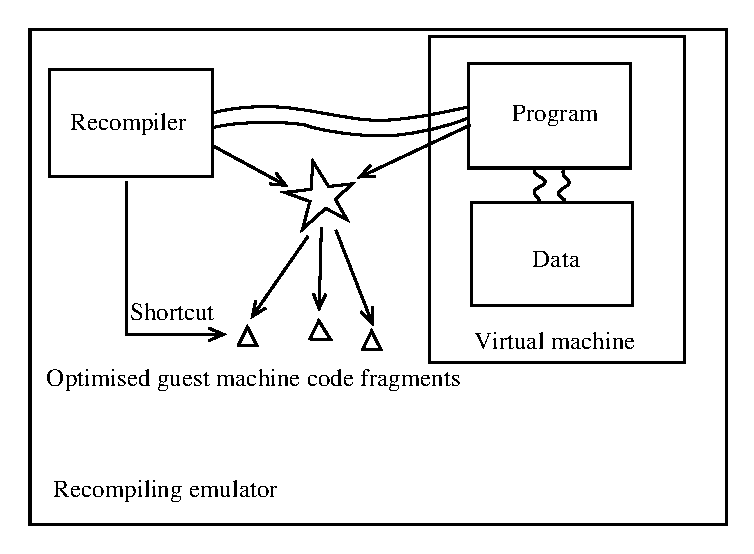
\includegraphics{recomp.ps}\end{center}
\vspace{0.3cm}


\subsection{Translation algorithm}

Given a piece of ARM code, we perform several passes on it in order
to translate it to IA-32 code. Firstly, since each ARM instruction
can be quite complicated, we translate to an intermediate representation%
\footnote{Note that one of the things Chameleon is trying to avoid is the need
for such an intermediate representation, by making the ISA \emph{itself}
the intermediate representation.%
}. which is much simpler and therefore easier to analyse. I will describe
this intermediate representation (ph2) below, since it is an important
part of the emulator, and helped form many of the ideas behind the
Chameleon instruction-set architecture%
\footnote{Apart from some of the nasty bits, which aren't necessary if an existing
processor isn't being emulated%
}.

The important things we need to do with the intermediate representation
are extracting and optimising control flow, performing register allocation
and doing IA-32 code generation.

Currently, the order of the passes required to do each of these is
as follows:

\begin{itemize}
\item Allocate constants. This means that ph2 variables which are loaded
with constants need not have physical IA-32 registers attached to
them later.
\item Optimise transitive branches. Rewrite the target of the first branch
which points directly to a second branch of compatible type to the
target of the second branch ({}``branch threading'').
\item Cull unused nodes. As possibly generated by the previous step, or
earlier in the ARM->ph2 translation step.
\item Depth-first search. Find `parent' nodes, start and finish times. Used
by the strongly-connected component code later.
\item Shuffle commits. Move commits as early as possible, to relieve register
pressure.
\item Find predecessors. This finds the inverse of the control flow graph.
\item Strongly-connected components. This finds strongly-connected components
in the control flow graph.
\item Fix-up flags \& predicates. Ensures that flags and control condition
codes are stored when needed, and culls unnecessary flag calculation
code.
\item Find spans. Find live variable ranges in ph2 code.
\item Source-destination alias. Where possible, alias the destination variable
to the source variable of the three-address operations used by ph2.
This is important for IA-32 code, where one of the source operands
for calculations is usually overwritten by the result.
\item Re-run span finder. The aliases from the previous stage alter the
variable liveness information.
\item Linear scan register allocation/code generation. Described below.
\item Insert load/store code. Cannot be known until after the previous stage
has completed.
\item Finish allocation. The way register allocation works means some variables
cannot be fully allocated until the end. This fixes them.
\item Flatten code. This takes abstract structure of IA-32 instructions,
and flattens them into contiguous code.
\end{itemize}
I will explain some of these stages further below, but first I will
describe the ph2 intermediate language.


\subsection{Intermediate representation}

The intermediate representation (ph2) is a three-address code, ie
instructions are of the form:

add \%7, \%3, \%4

\%3, \%4 and \%7 represent variables. \%3 and \%4 are source operands,
\%7 is the destination. Each of the operations available are simple
(simpler than many RISC chips). ARM code in particular can be quite
expressive, allowing immediate and shifted operands for data-processing
instructions, predicated execution of instructions, etc. Complex ARM
instructions are broken up into many ph2 instructions. Additionally,
the ARM instruction encoding at a bit level is fairly involved, and
ph2's encoding is very simple. This aids code analysis greatly, and
has been very influential on the Chameleon architecture.


\subsubsection{SSA}

By convention, ph2 is always written in static single assignment (SSA)
form. During the ARM->ph2 translation phase, this conversion is performed
by performing \emph{register renaming} in much the same way as a modern
superscalar processor does. This form allows certain types of optimisation
to be performed very quickly and easily (linear time vs quadratic
time).


\subsubsection{Control flow}

Ph2 instructions are grouped into blocks. There is no explicit branch
instruction, but instead each block has a condition type, and pointers
to a `true' block and a `false' block. It is not necessary to exactly
mirror all of the condition-code flags which the source machine code
used, since the host machine's native control-flow logic is used instead.
Of course, flags must be calculated correctly before control returns
to the interpretive emulator.

In more detail, on the ARM architecture, as on many others, flow control
is achieved using condition codes, which are combinations of particular
flags in some status register. For example, a piece of code might
want to jump somewhere if one register is greater than or equal to
another register:

cmp r4,r5

bge somewhere

The first instruction sets four flags, named Z (zero), N (negative),
V (overflow) and C (carry). The second tests a combination of those
flags for the ``greater-than or equal'' condition, which is defined
by ``N set and V set, or N clear and V clear'', or more concisely
as ``N==V''.

The two architectures in question (ARM and IA-32) both employ flags
for controlling flow like this, but have quite different semantics
for setting and testing those flags. On the ARM for example, setting
flags is optional for ALU operations, and any instruction may be conditionally
executed. In IA-32, virtually all instructions unconditionally set
(or in some cases corrupt) the processor flags. Nevertheless, we can
still utilise the native processor's flag-calculation logic in recompiled
code, although great care must be taken.

One approach (that used in an earlier version of the emulator \cite{Brown 00}),
is to save and restore flags individually, on-demand, in recompiled
code. This was proven to work adequately, but produced bulky and slow
code. The reason is mainly a shortcoming of IA-32, which makes it
particularly difficult to alter individual bits corresponding to the
S (sign), Z (zero) and O (overflow) flags in the flags register. The
code sequence used -- not necessarily the best -- took between 9 and
18 instructions to restore between one and four bits. When this was
multiplied by the number of times such an operation was necessary
in a chunk of code, this meant a fairly large proportion of code was
dedicated to this type of code.


\subsubsection{Condition-code abstraction}

A better approach is to group flags forming a condition code together,
and treat them as an atomic unit (IA-32 provides convenient set\emph{xx}
instructions which allow you to do just that). This means that the
state of the flags is not mirrored exactly in recompiled code, and
the on-demand scheme can no longer be utilised. Instead, when we encounter
a conditional branch (say), we scan the ph2 representation backwards
(over block boundaries if necessary) until we find the instruction
which last altered the flags corresponding to the relevant condition
code. Then we insert an instruction which saves that condition code
into a predicate buffer, and use that value rather than the condition
flags when we decide whether to take the branch or not. Additionally,
the pass which does this removes any redundant flag calculation%
\footnote{Actually flag saving, since on IA-32 flags are calculated whether
you want them to be or not. It's the code to store the flags to memory
that takes up space.

As you might imagine, the subtleties of this approach are more involved
than I'm describing here. ARM and IA-32 treat the carry flag in an
inverse sense from one another as the result of subtraction (including
comparison) operations for instance, so we must always ensure that
we're using the correct sense. If a compound condition code, ie, the
unsigned lower-or-same (carry-clear or zero-set) test is used, then
the \emph{host} machine's sense of the carry flag must be used. Contrariwise,
If the carry-set (unsigned higher-or-same) test is used, the \emph{guest}
machine's sense of the carry flag must be used.%
} code.

To avoid all this headache, Chameleon does not use an implicit flag
word, instead relying on general-purpose registers to hold predicate
values.


\subsection{Modified Linear Scan}

Linear Scan is a fast register allocation technique \cite{PS}, developed
as an alternative to allocation by graph colouring \cite{Chaitin et al}
for situations where compile-time is at a premium. Unfortunately in
its basic form it is inconvenient for use in a dynamic recompilation
system since information it requires whilst working is needed during
other stages of code generation. First I'll explain how it normally
works, then I'll describe my modification. (An earlier version of
the emulator used an ad-hoc register allocation technique similar
in spirit to ``binpacking\char`\"{} \cite{THS 98})

The algorithm works as follows. It is assumed that program instructions
can be laid out in some order, for instance the order in which the
intermediate representation is laid out in memory or the order arising
from a depth-first search.

The intermediate representation is scanned and from it a set of \emph{live
intervals} for variables is inferred. Two live intervals interfere
if they overlap. Given \emph{R} available registers and a list of
live intervals, the linear scan algorithm must allocate registers
to as many intervals as possible, such that no two overlapping intervals
are assigned the same register. If $n>R$ live intervals overlap at
any point, at least $n-R$ of them must reside in memory.

The number of overlapping intervals only changes at the start and
end of an interval. Live intervals are stored in an list sorted by
increasing start point, so the algorithm can progress quickly by skipping
from one start interval to the next.

At each step, the algorithm maintains a list of \emph{active} live
intervals, which have been assigned to registers. This list is kept
in order of increasing end point. For each new interval, the algorithm
scans \emph{active} and removes any `expired' intervals which are
no longer pertinent to the current position in the source program,
leaving such interval's registers free for reallocation. Since this
list is stored in increasing end-point order, scanning can stop when
an end-point greater than the current new start point has been encountered.

The worst case scenario, where the active list has length $R$ and
no intervals have been expired, is resolved by choosing one of the
intervals from \emph{active} or the new start interval. As a heuristic,
the interval which ends furthest from the current point is spilled
to memory. This information can be found quickly since \emph{active}
is sorted by increasing end point. Further analysis is available in
\cite{PS}.

Due to the context from which the `source' code is obtained in our
dynamic recompilation environment, any memory access instruction (load
or store) can cause a data abort exception. If this happens, we must
be able to recover the original processor state%
\footnote{There is no practical opportunity for returning control to the block
which caused the exception and allowing the state to be recovered
gracefully, since the true machine state must be available to the
exception handler anyway%
}. Up to $R$ ARM registers may reside in IA-32 registers at a point
in a recompiled block. If an exception occurs, these must be spilled
back to memory before the exception handler is invoked. This set of
registers is known as linear scan is in operation, so rather than
wastefully store the data somewhere, code is generated at the same
time as registers are allocated (a similar early code-generation philosophy
is advocated in \cite{Appel 98}).

The problem then is that an interval used by code which has already
been generated cannot easily be spilled without altering already-generated
code in which that interval was live. The solution to this is to generate
code in an abstracted form, with mutable `slots' for the operands.
These slots are only finalised when the linear scan algorithm has
completed.

This approach has additional benefits where a non-orthogonal instruction
set is concerned (such as on IA-32), in that if a particular register
is needed for some operation, then:

\begin{itemize}
\item As we're generating code at the same time as allocating registers,
we can tell if particular registers are needed in a timely way
\item The set of allocated registers can be `shuffled around' to enable
the difficult instruction to use the registers it wants.
\end{itemize}
Note that even on `clean' architectures, the procedure call convention
usually passes and returns values in particular registers.


\subsection{Instruction Selection}

We generate code by simply choosing IA-32 instructions which correspond
to ph2 instructions one at a time (the earlier incarnation of the
emulator used a complicated tree-based matching method). Code is generated
indirectly via an abstraction layer as mentioned above, which performs
a similar task to a text-source assembler in choosing instruction
variants for different operand types, but also knows about which instructions
set up and destroy condition-code flags.


\subsection{Flattening Code}

Given a graph of basic blocks, there are any number of ways to lay
out those blocks into a linear instruction stream (and insert instructions
to control the flow of execution). My algorithm is fairly ad-hoc,
and as yet has not been subjected to rigourous testing. A priority
queue is used to decide which block to output next. The `true' and
`false' blocks for each block by default are added to this queue after
that block has been generated. Their priorities are increased if they
are:

\begin{itemize}
\item Part of the same strongly-connected component as the current block
(to try to keep loops together)
\item For the true block, if there is no false block (to try to keep straight-line
code together)
\item In the future, a weighting might be added depending on how often branches
were taken/not taken in the profiling of the original code before
translation.
\end{itemize}
The rationale being that spatially-adjacent code accesses are more
likely to be accessed close together in time.


\section{Summary}

In this report, I have described various pieces of work related to
dynamic optimisation. Additionally, I have described two projects,
one on the drawing board (Chameleon) and one partly implemented (ARM->IA-32
recompiling emulator).

\begin{thebibliography}{10}
\bibitem{CL 96}R. Cohn and G. Lowney, {}``Hot Cold Optimization of Large Windows/NT
Applications,'' Proc. of the 29th Annual Int. Symposium on Microarchitecture,
pages 80-89, December 1996.
\bibitem{2}R. Cohn, D. Goodwin, P. G. Lowney and N. Rubin, {}``Spike: An Optimizer
for Alpha/NT Executables,'' The USENIX Windows NT Workshop Proceedings,
Seattle, Wash. (August 1997): 17-24.
\bibitem{BL 94}T. Ball and J. Larus, {}``Optimally Profiling and Tracing Programs,''
ACM Transactions on Programming Languages and Systems, 16(3):1319-1360,
July 1994.
\bibitem{LL 96}Peter Lee and Mark Leone, {}``Optimizing ML with Run-Time Code Generation,''
In ACM SIGPLAN '96 Conference on Programming Language Design and Implementation,
Philadelphia, May 1996.
\bibitem{Engler 96}Dawson R. Engler, {}``A Retargetable, Extensible, Very Fast Dynamic
Code Generation System,'' SIGPLAN Conference on Programming Language
Design and Implementation (PLDI '96), Philadelphia, PA, May 1996.
\bibitem{KP 95}Wayne Kelly and William Pugh, {}``A Unifying Framework for Iteration
Reordering Transformations,'' ???
\bibitem{PS}Massimiliano Poletto and Vivek Sarkar, {}``Linear Scan Register Allocation,''
ACM Transactions on Programming Languages and Systems, Volume 21,
Issue 5 (Sept. 1999), pp 895-913.
\bibitem{Chaitin et al}Chaitin, G. J., Auslander, M. A., Chandra, A. K., Cocke, J., Hopkins,
M. E., and Markstein, P. W., {}``Register allocation via coloring,''
Computer Languages 6, 47-57, 1981
\bibitem{THS 98}Traub, O., Holloway, G., and Smith, M. D., {}``Quality and speed
in linear-scan register allocation,'' Proc. ACM SIGPLAN '98 Conference
on Programming Language Design and Implementation, 1998
\bibitem{Michie 68}Michie, D., {}``Memo Functions and Machine Learning,'' Nature 218,
pp. 19-22, 1968.
\bibitem{Brown 00}Brown, J., {}``ARMphetamine: A Dynamically Recompiling ARM Emulator,''
Final-year dissertation, University of Cambridge, 2000.
\bibitem[12]{Appel 98}Appel, Andrew W., {}``Modern Compiler Implementation in ML,'' Cambridge
University Press, 1998
\bibitem{key-1}Chen, J. B., {}``Improving Instruction Locality with Just-In-Time
Code Layout,'' 1997 USENIX Windows NT Workshop.
\bibitem{Hazelwood}Hazelwood, K. M., {}``Dynamic Optimization Infrastructure and Algorithms
for IA-64,'' Master of Science thesis, Raleigh, 2000.
\bibitem{key-3}Kistler, T. P., {}``Continuous Program Optimization,'' Ph.D. thesis,
University of California, Irvine, 2000.\end{thebibliography}

\end{document}
